Рассмотрим вышеупомянутые алгоритмы сортировки. Для удобства изложения сути алгоритмов, будем рассматривать сортировку по неубыванию. Алгоритмы сортировки других порядков могут быть получены заменой условия сравнения.

\section{Сортировка пузырьком}
Алгоритм сортировки пузырьком основывается на следующем действии. Массив проссматривается от 0 до N-2 элемента, и в случае, если текущий элемент массива больше следующего, они меняются местами. Таким образом, после первого прохода в конце массива окажется максимальный элемент, после второго - два максимальных, и так далее до полного упорядочивания массива.

Схема алгоритма приведена на рисунке 2.1.
\begin{figure}[h]
	\begin{center}
		{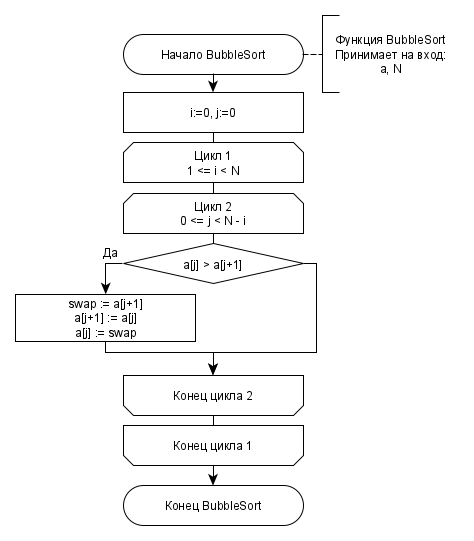
\includegraphics[width = 17cm]{Bubble}}
		\caption{Сортировка пузырьком}
	\end{center}
\end{figure}


\section{Сортировка расчёской}
Алгоритм является модификацией вышеописаного алгоритма. Основной идеей является то, что "почти упорядоченый" массив можно отсоритровать быстрее, чем неупорядоченый вовсе. Поэтому, сначала сортируются множества элементов массива расположеных друг от друга на расстоянии $ Step $. Следующим шагом сортировка происходит по $ \frac{Step}{2} $ и т.д. до шага в 1. Сортировка подмассивов происходит по алгоритму пузырька.

Первоначально $Step = N/\alpha$, где $\alpha$ - фактор уменьшения. Наиболее оптимальное значение этого фактора равно $\dfrac{1}{1-e^{-\phi}} \approx 1.247$, где $\phi$ - золотое сечение. Следующий шаг считается как $Step/\alpha$ до тех пор, пока на станет равным 1.

Схема алгоритма приведена на рисунке 2.2.
\begin{figure}[h]
	\begin{center}
		{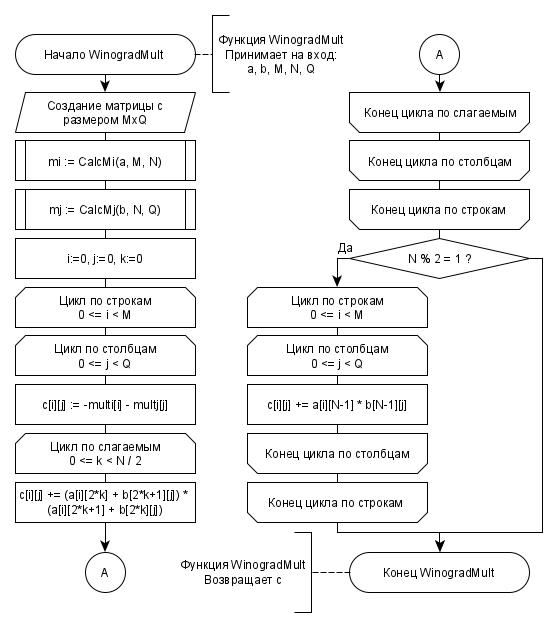
\includegraphics[scale = 0.8]{Winograd1}}
		\caption{Алгоритм Винограда}
	\end{center}
\end{figure}


\section{Сортировка слиянием}
Идея алгоритма заключается в том, что достаточно эффективно производится операция слияния (т.е. создания из двух массивов одного) при условии, что оба сливаемых массива уже упорядочены. Алгоритм разбивает массив на два подмассива, после чего применяет к ним ту же операцию, до тех пор, пока длина массива не станет меньше 3. После завершения сортировки подмассивов производится построение упорядоченного массива их слиянием.

Схема алгоритма приведена на рисунке 2.3.
\begin{figure}[h]
	\begin{center}
		{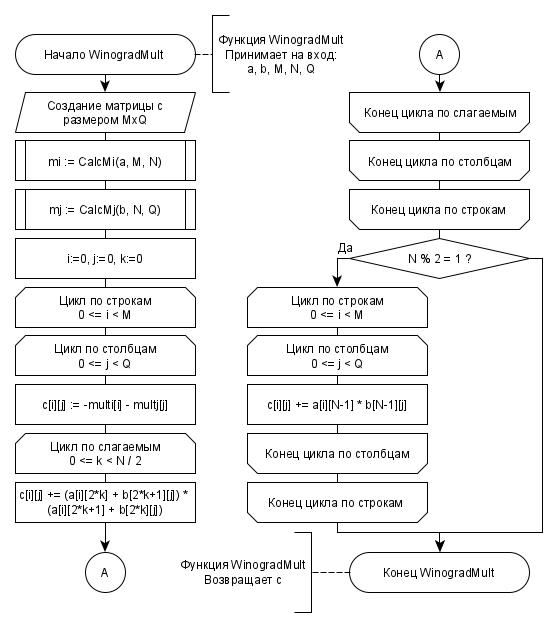
\includegraphics[scale = 0.8]{Winograd1}}
		\caption{Алгоритм Винограда}
	\end{center}
\end{figure}


\section{Требования к программному обеспечению}
Для полноценной проверки и оценки алгоритмов необходимо выполнить следующее.
\begin{enumerate}
	\item Обеспечить возможность консольного ввода массива и выбора алгоритма сортировки. Программа должна вывести отсортированный массив.
	\item Реализовать функцию замера процессорного времени, затраченного функцией. Для этого также создать возможность ввода размера массива, на котором будет выполнен замер.
\end{enumerate}


\section{Заготовки тестов}
При проверке алгоритмов необходимо будет использовать следующие классы тестов:
\begin{itemize}
	\item массив размером 1;
	\item массив одинаковых элементов;
	\item упорядоченный массив;
	\item массив упорядоченный в обратном порядке.
\end{itemize}



